%!TEX root = ../paper.tex
\begin{figure*}
	\todo[inline]{Split into two seperate figures? The results are not that interesting to see side by side.}
	\centering
	%!TEX root = ../paper.tex

% Ferdosi 2, MBE
\begin{subfigure}{0.23\textwidth}
	\centering
	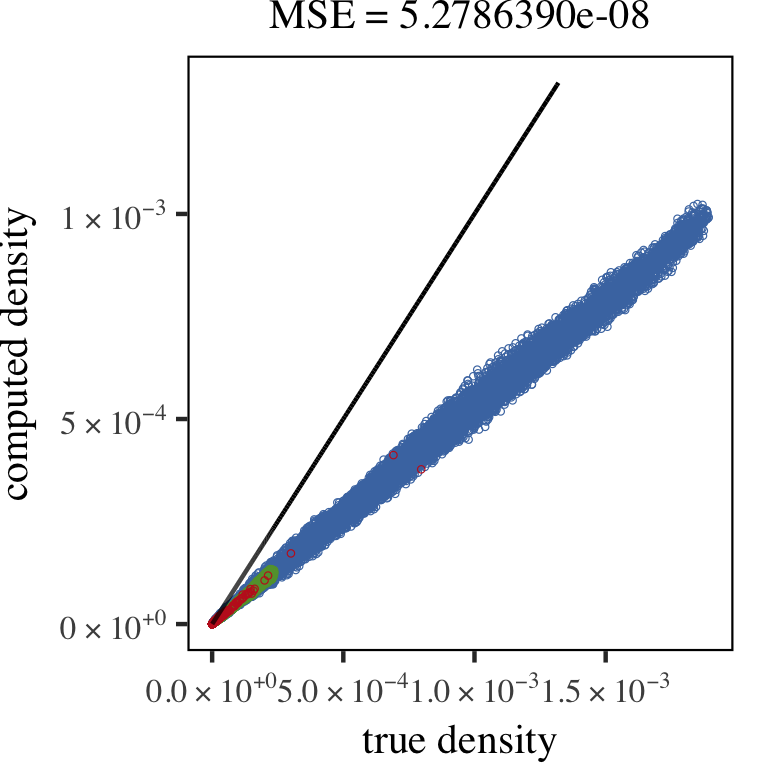
\includegraphics[keepaspectratio=true, width=\textwidth, height=0.23\textheight]{result/img/all/results_ferdosi_2_60000_mbe_silverman}
	\caption{Set \ferdosiTwo, \mbe}
	\label{fig:4:results:mbe:ferdosi2}
\end{subfigure}
% Baakman 2, MBE
\begin{subfigure}{0.23\textwidth}
	\centering
	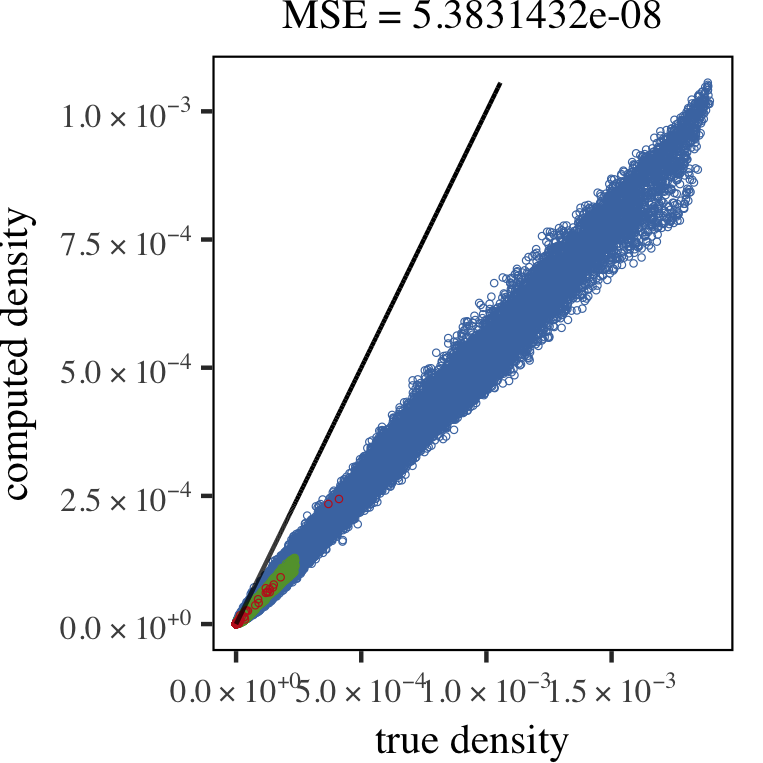
\includegraphics[keepaspectratio=true, width=\textwidth, height=0.23\textheight]{result/img/all/results_baakman_2_60000_mbe_silverman}
	\caption{Set \baakmanTwo, \mbe}
	\label{fig:4:results:mbe:baakman2}
\end{subfigure}
% Ferdosi 3, MBE
\begin{subfigure}{0.23\textwidth}
	\centering
	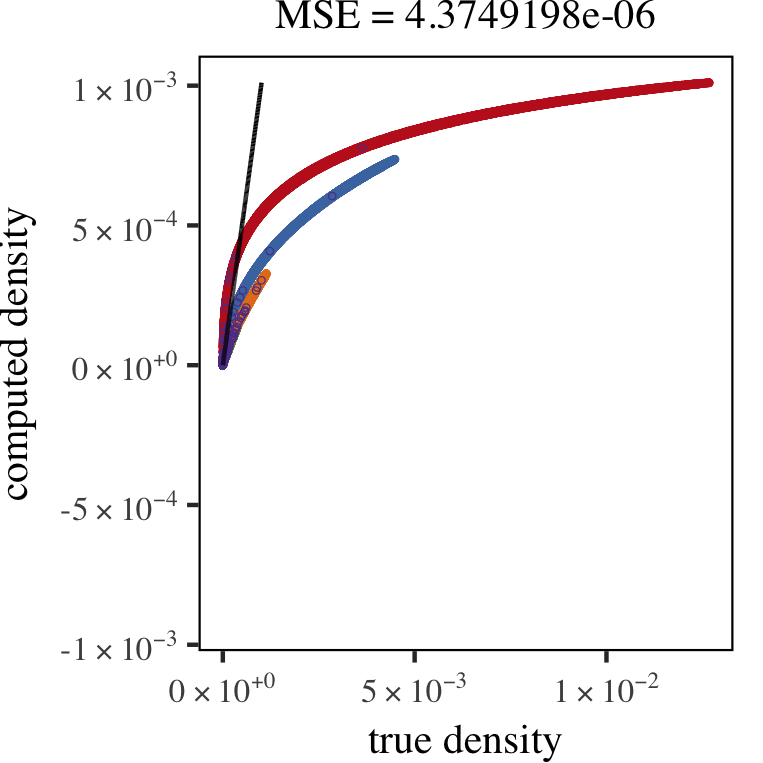
\includegraphics[keepaspectratio=true, width=\textwidth, height=0.23\textheight]{result/img/all/results_ferdosi_3_120000_mbe_silverman.png}
	\caption{Set \ferdosiThree, \mbe}
	\label{fig:4:results:mbe:ferdosi3}
\end{subfigure}
% Baakman 3, MBE
\begin{subfigure}{0.23\textwidth}
	\centering
	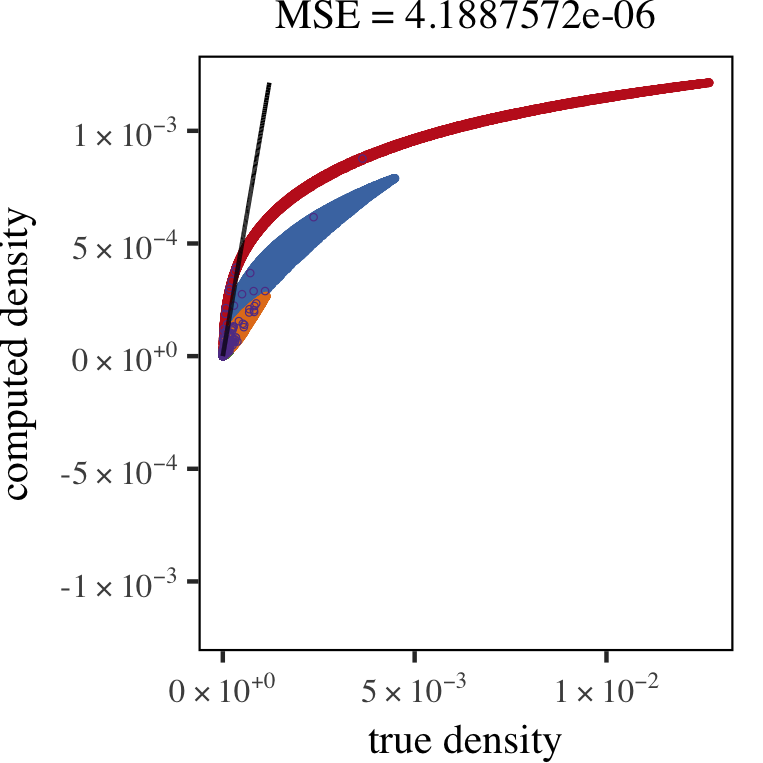
\includegraphics[keepaspectratio=true, width=\textwidth, height=0.23\textheight]{result/img/all/results_baakman_3_120000_mbe_silverman}
	\caption{Set \baakmanThree, \mbe}
	\label{fig:4:results:mbe:baakman3}
\end{subfigure}	
% Ferdosi 2, SAMBE
\begin{subfigure}{0.23\textwidth}
	\centering
	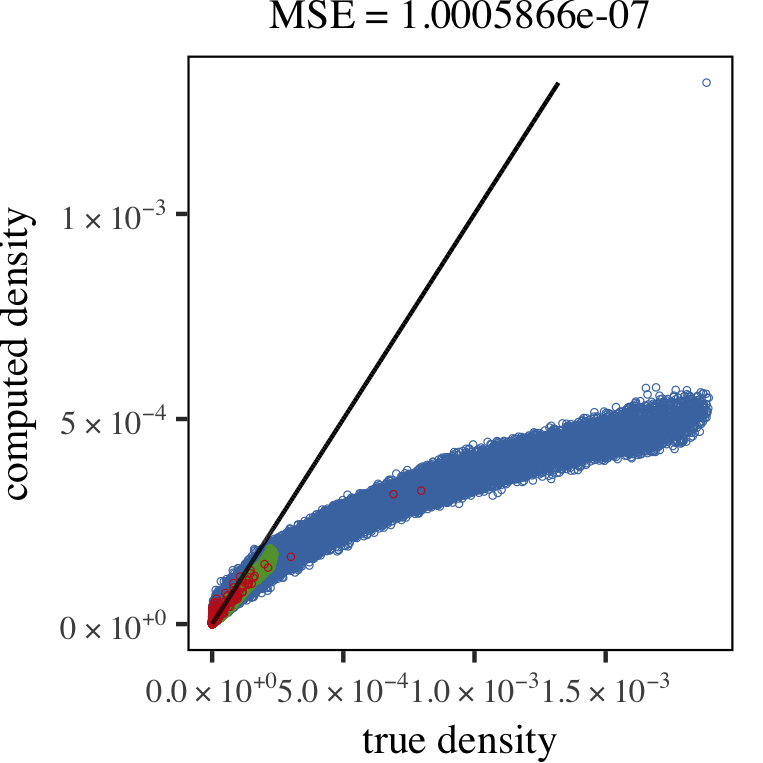
\includegraphics[keepaspectratio=true, width=\textwidth, height=0.23\textheight]{result/img/all/results_ferdosi_2_60000_sambe_silverman}
	\caption{Set \ferdosiTwo, \sambe}
	\label{fig:4:results:sambe:ferdosi2}
\end{subfigure}
% Baakman 2, SAMBE
\begin{subfigure}{0.23\textwidth}
	\centering
	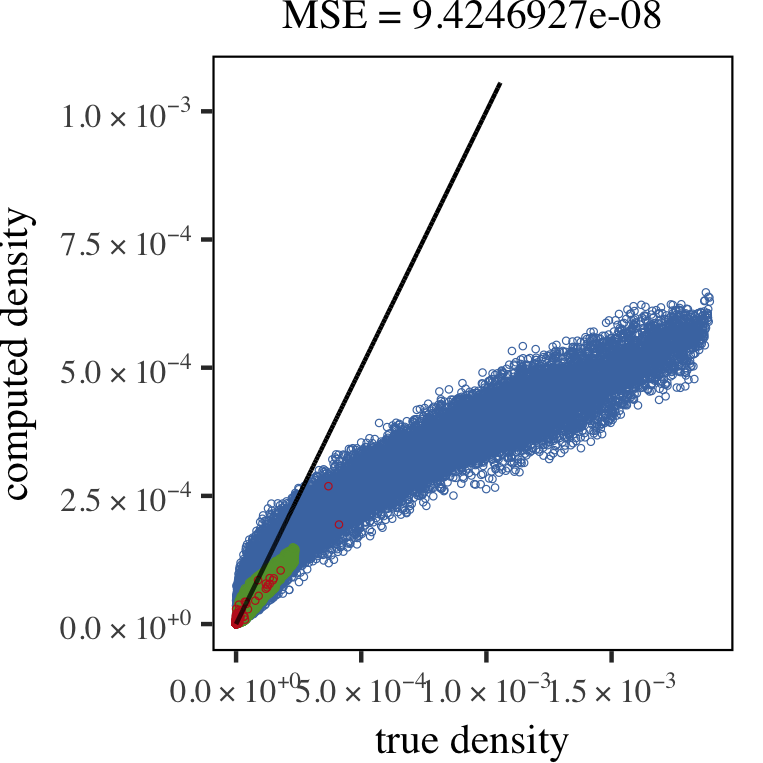
\includegraphics[keepaspectratio=true, width=\textwidth, height=0.23\textheight]{result/img/all/results_baakman_2_60000_sambe_silverman}
	\caption{Set \baakmanTwo, \sambe}
	\label{fig:4:simulated:datasets:sambe:baakman2}
\end{subfigure}
% Ferdosi 3, SAMBE
\begin{subfigure}{0.23\textwidth}
	\centering
	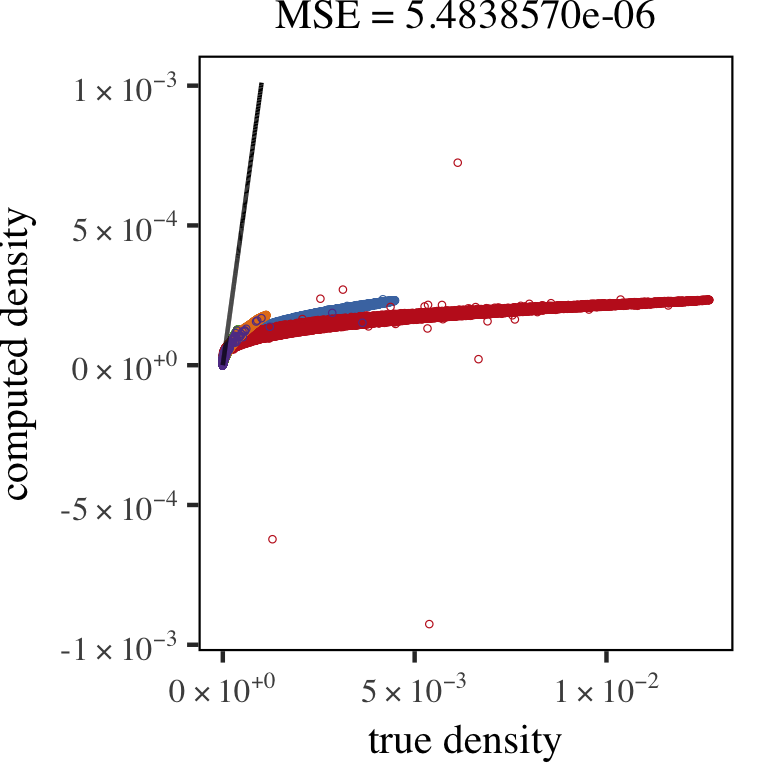
\includegraphics[keepaspectratio=true, width=\textwidth, height=0.23\textheight]{result/img/all/results_ferdosi_3_120000_sambe_silverman}
	\caption{Set \ferdosiThree, \sambe}
	\label{fig:4:simulated:datasets:sambe:ferdosi3}
\end{subfigure}
% Baakman 3, SAMBE
\begin{subfigure}{0.23\textwidth}
	\centering
	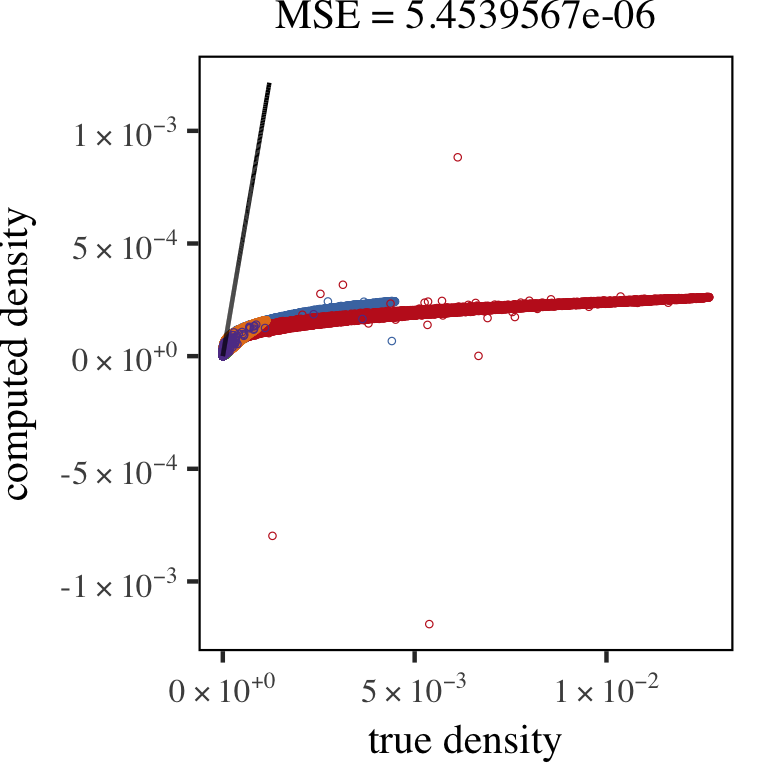
\includegraphics[keepaspectratio=true, width=\textwidth, height=0.23\textheight]{result/img/all/results_baakman_3_120000_sambe_silverman}
	\caption{Set \baakmanThree, \sambe}
	\label{fig:4:results:sambe:baakman3}
\end{subfigure}	
	\caption{Comparative plots for dataset \ferdosiTwoNum, \ferdosiThreeNum, \baakmanTwoNum, and \baakmanThreeNum.}
	\label{fig:results:multiSphere:comparativePlots}
\end{figure*}

\begin{table}
	\todo[inline]{Rewrite caption}
	\centering
	%!TEX root = ../paper.tex
\begin{tabular}{l*{2}{S[scientific-notation=true, round-mode=places,round-precision=3]}}
\toprule
~ 				& \multicolumn{2}{c}{Estimator}\\ \cmidrule{2-3}
Set				& {\mbe}					& {\sambe}	\\
\midrule
\ferdosiTwo		& 0.0	&  0.0 \\
\baakmanTwo		& 0.0	&  0.0 \\	
\ferdosiThree	& 0.0	&  0.0 \\		
\baakmanThree	& 0.0	&  0.0 \\	
\bottomrule
\end{tabular}
	\caption{The mean squared error of the known densities and the densities as estimated by the Modified Breiman Estimator (\mbe) and the shape-adaptive MBE (\sambe), respectively, for the datasets containing a single Gaussian.} 	
	\label{tab:results:multiSphere:mse}
\end{table}

In this section we present the results of the two estimators on dataset \ferdosiTwo, \baakmanTwo, \ferdosiThree, \baakmanThree, \ie the datasets that contain more than one Gaussian.

% Ferdosi 2 & Baakman 2
	% MSE
	\todo[inline]{Discuss MSE and Plot}
	\todo[inline]{Difference between noise and gaussians?}	

	% Plots

% Ferdosi 3 & Baakman 3
	% MSE
	\todo[inline]{Discuss MSE and Plot}
	\todo[inline]{Difference between noise and gaussians?}	

	% Plots

% General
	\todo[inline]{General observation?}
	\todo[inline]{What is the influence of the density of Gaussian?}